\documentclass[../../main.tex]{subfiles}
\begin{document}
\subsubsection{Gleiserkennung}
Ein Beschleunigungssensor für die Erfassung der Fahrdaten ist bereits in der Aufgabenstellung vorgeschrieben.
Um aber eine ideale Regelung zu ermöglichen wird zusätzlich eine Gleiserkennung implementiert. Mitwelcher schon im vorraus
erkennt werden kann ob eine Kurve bevorsteht oder ob sich der Hochgeschwindigkeitszug auf einer geraden befindet.
Während der Konzept Phase wurden verschiedene Verfahren evaluiert und zum Teil ausprobiert. Jedoch gab es keine Lösung welche zusätzlich zur Richtung noch den Radius
der Kurve bestimmen kann. Die Momentane Lösung welche angestrebt wird kann also nur sagen ob es Geradeaus, nach Links oder nach Rechts geht.
Diese Information wird in den Regelungskreis eingespiesen, welcher dadurch auf die maximale Geschwindikeit die im engsten schienen Radius möglich ist
herunterreglet. Anschliessend wird mithilfe des Beschleunigungssensor versucht an das Limit der Zentripedalkraft zu regeln. Somit kann die
bestmögliche Regelung implementiert werden ohne genauere Angaben zum aktuellen Kurvenradius zu haben.
Mehr Details zum Regelkreis und dem Ganzen Ablauf sind im unter \ref{ablauf} zu finden.

\subsubsection{Verfahren}
Im folgenden Diagramm wird die Architektur der Steuerungssoftware aufgezeigt
\begin{figure}[H] %Architektur mit Middleware
    \centering
    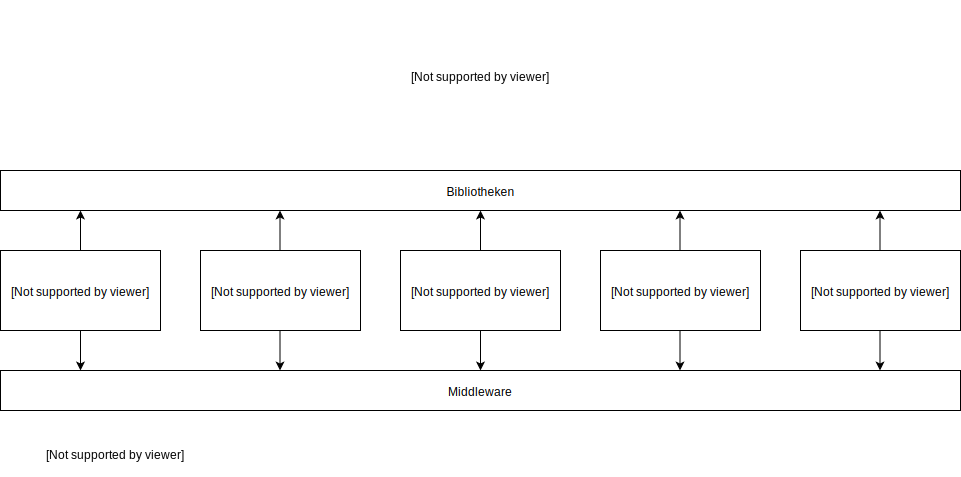
\includegraphics[width=1.0\textwidth]{../../drawings/ArchitekturDiagramm/SW_Architektur_Middleware.png}
    \caption {Software Architektur Middleware. Gezeichnet mit https://draw.io}
\end{figure}

\end{document}